\section{Partitioning for Spark}

%$$$$$$$$$$$$$$$$$$$$$$$$$$$$$$$$$$$$$$$$$$$$$$$$$$$$$$$$$$$$$$$$$$$$$$$$$$$$$$$$
%$$$$$$$$$$$$$$$$$$$$$$$$$$$$$$$$$$$$$$$$$$$$$$$$$$$$$$$$$$$$$$$$$$$$$$$$$$$$$$$$
% 일반적인 매니코어 또는 Scale-server의 scalability 대한 설명과 이번장에 대한 설명
%$$$$$$$$$$$$$$$$$$$$$$$$$$$$$$$$$$$$$$$$$$$$$$$$$$$$$$$$$$$$$$$$$$$$$$$$$$$$$$$$
The reason for requiring partitioning method is that
spark library and runtime engine can be bottlenect by GC and memory latency
because Spark have not been considers scale-up environment.
%However, modification of the spark internals library and the runtime engine is
%difficult.
Thus, we use the docker container-based partitioning method to eliminate GC and
memory latency overheads. 
%The fundamental solution for scaling spark make a new designed spark
%libary and runtime engine scale for scale-up server.
This section explains design aspects of our docker container-based
partitioning method to solve GC and memory latency.

\subsection{Design Consideration}

%$$$$$$$$$$$$$$$$$$$$$$$$$$$$$$$$$$$$$$$$$$$$$$$$$$$$$$$$$$$$$$$$$$$$$$$$$$$$$$$$
%$$$$$$$$$$$$$$$$$$$$$$$$$$$$$$$$$$$$$$$$$$$$$$$$$$$$$$$$$$$$$$$$$$$$$$$$$$$$$$$$
% 파티션닝의 장점 1: GC의 serialization 되는 부분을 줄인다.
%$$$$$$$$$$$$$$$$$$$$$$$$$$$$$$$$$$$$$$$$$$$$$$$$$$$$$$$$$$$$$$$$$$$$$$$$$$$$$$$$
\ifkor
%파티션닝 방법이 필요한 가장 큰 이유는 GC의 영향 때문이다. 
The major problem of Spark scalability is GC, so partitioning approch is needed.
Indeed, GC leads to many of the advantages of high-level languages becuase of
an increase in productivity, while it is a double-edged sword because
GC pauses can cause serilizaed operation and requests to take unacceptable long
times.
Thus, reducing GC pause time may lead to high performance scalability,
and minialized CPU counts can mitigate GC pause time[].
Therefore, the first design consideration of scale partitioning is to minimize GC
pause times.
\else

\fi

%$$$$$$$$$$$$$$$$$$$$$$$$$$$$$$$$$$$$$$$$$$$$$$$$$$$$$$$$$$$$$$$$$$$$$$$$$$$$$$$$
%$$$$$$$$$$$$$$$$$$$$$$$$$$$$$$$$$$$$$$$$$$$$$$$$$$$$$$$$$$$$$$$$$$$$$$$$$$$$$$$$
% 파티션닝의 장점 2: DRAM access latency를 최대화 한다.
%$$$$$$$$$$$$$$$$$$$$$$$$$$$$$$$$$$$$$$$$$$$$$$$$$$$$$$$$$$$$$$$$$$$$$$$$$$$$$$$$
\ifkor
%파티션닝 방법이 필요한 두번째 이유는 DRAM access latency 때문이다. 
The second design consideration is locality issues because of NUMA archtecture
DRAM access latency.
For example, threads are scheduled by the OS to execute on any core. When
the thread is migrated to different memory area, the thread may accesse
remote memory.
Partitioning aprroach can prevent to migrate other socket's core.
Indeed, the modern operating systems(Linux) has a NUMA balancing feature for
enhancement of memory locality, but partitioning method can more superial
performance regarding the large scale-up server(8 socket)[](see section 2).
\else

\fi

%$$$$$$$$$$$$$$$$$$$$$$$$$$$$$$$$$$$$$$$$$$$$$$$$$$$$$$$$$$$$$$$$$$$$$$$$$$$$$$$$
%$$$$$$$$$$$$$$$$$$$$$$$$$$$$$$$$$$$$$$$$$$$$$$$$$$$$$$$$$$$$$$$$$$$$$$$$$$$$$$$$
% 파티션닝의 장점 3: DRAM access latency를 최대화 한다.
% Linux kernel scalability (lock, cache cohearnci, scheduler)등등 OS 노이즈에 대한 설명
%$$$$$$$$$$$$$$$$$$$$$$$$$$$$$$$$$$$$$$$$$$$$$$$$$$$$$$$$$$$$$$$$$$$$$$$$$$$$$$$$
\ifkor
In addition to GC and NUMA effect, operating systems noise can pose scalability
bottlenct because it designed for shared-memory system;therefore, the next
design consideration is to avoid operating system noise.
For example, Single address sapce sharing problem[][][][] between multi-thread
applications on JVM, scheduer bottlenct by load balancer[][], and cache
comunication bottlenct[][] are major problems in manycore scale-up server
operating system.
This problem cause by sharing resource, so our approach can solve from these
resource contention by using partitiong approch.
\else

\fi

%$$$$$$$$$$$$$$$$$$$$$$$$$$$$$$$$$$$$$$$$$$$$$$$$$$$$$$$$$$$$$$$$$$$$$$$$$$$$$$$$
%$$$$$$$$$$$$$$$$$$$$$$$$$$$$$$$$$$$$$$$$$$$$$$$$$$$$$$$$$$$$$$$$$$$$$$$$$$$$$$$$
% 스파크는 결국 : shared memory system -> distributed system 처럼해야한다. 
%$$$$$$$$$$$$$$$$$$$$$$$$$$$$$$$$$$$$$$$$$$$$$$$$$$$$$$$$$$$$$$$$$$$$$$$$$$$$$$$$
\ifkor
To satisfy these factors such as GC, NUMA and operating system
bottlenct cause by shared-memory system, Spark on scale-up server should work
as distributed system concept. 
Therefore, we use partitioning approch for shared-memory system and it is dealt
with as the distributed-system big data analytics frameworks thereby eliminating
GC and memory access overheads.
We make shared resource to small size group as much as possible; as result of,
the small size cpu groups can mitigate the thread serialized problem cased by GC
pause time, and these group may only accees to local NUMA memory.
%따라서 본 연구는 메모리와 CPU를 적은 수의 CPU와 메모리로 파티션닝을 하여 마치 shared memory 시스템을 distributed
%system 처럼 동작하도록 제안 한다.
%스파크 워커들은 모두 독립적인 cpu와 memory를 할당받아 최대한 thread간의 공유메모리와 remote
%memory에 접근을 막도록 하였다.
\else

\fi



%$$$$$$$$$$$$$$$$$$$$$$$$$$$$$$$$$$$$$$$$$$$$$$$$$$$$$$$$$$$$$$$$$$$$$$$$$$$$$$$$
%$$$$$$$$$$$$$$$$$$$$$$$$$$$$$$$$$$$$$$$$$$$$$$$$$$$$$$$$$$$$$$$$$$$$$$$$$$$$$$$$
% 스파크는 적당한 파티션닝이 중요하다. 
%$$$$$$$$$$$$$$$$$$$$$$$$$$$$$$$$$$$$$$$$$$$$$$$$$$$$$$$$$$$$$$$$$$$$$$$$$$$$$$$$
\ifkor
The final design consideration is straggler tasks problem. 
If too small size partitioning may reduce GC and NUMA remote access, its benefit
does not come for free because it may cause straggler tasks problem[][].
Thus, in order to scale Spark performance scalability,  depending on
partitioning size.
\else

\fi


\subsection{Towards a Container-based Framework}

\begin{figure}[h]
  \begin{center}
     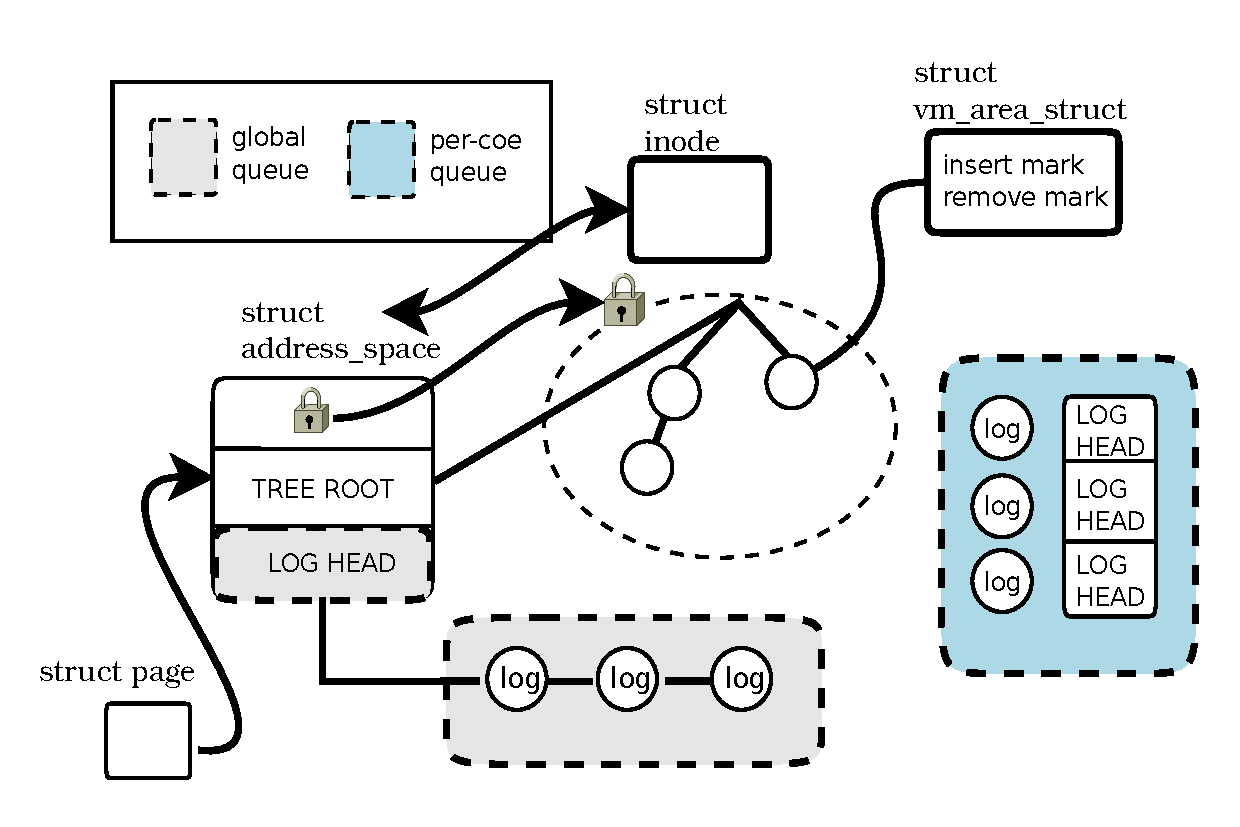
\includegraphics[width=0.5\textwidth]{fig/jaildocker}
  \end{center}
  \caption{Overview of the docker contrainer-based
  partitioning}
  \label{fig:basic}
\end{figure}

%$$$$$$$$$$$$$$$$$$$$$$$$$$$$$$$$$$$$$$$$$$$$$$$$$$$$$$$$$$$$$$$$$$$$$$$$$$$$$$$$
%$$$$$$$$$$$$$$$$$$$$$$$$$$$$$$$$$$$$$$$$$$$$$$$$$$$$$$$$$$$$$$$$$$$$$$$$$$$$$$$$
% 제안하는 구조 framework 설명
%$$$$$$$$$$$$$$$$$$$$$$$$$$$$$$$$$$$$$$$$$$$$$$$$$$$$$$$$$$$$$$$$$$$$$$$$$$$$$$$$
\ifkor
This section describes our vision that will accommodate the previous
mentioned design consideration.
Our proposed scaleble partitiong framework is figure~\ref{fig:basic} with the
necessary features.
The left side of figure shows our proposed framework, and the right side of
figure shows isolated docker containers and per-socket cpu with memory.
 %그림의 좌측은 우리가 제안하는 방법에 대한 프레임 워크를 보여주며, 오른쪽은 
%파티션된 docker container들과 native로 동작하기 위한 구조를 보여주며, 마지막으로
%소켓단위의 DRAM을 보여준다.

%The main components of the framwork are the decistion engine.
Decision engine is one of the most important features
since every partitioning regarding Spark system workers are based
on our decision engine compnent.
% 만약 사용 가능한 코어수가 작으면 SPARK는 적은 코어에서는 그림 <x-x>와 같이
%Scalabe하므로 파티션된 도커 컨테이너에서 수행하지 않고, 그냥 Native로 수행한다.
Our simplified algorithm of the decision engine is that if available cores are
less than pre-defined thrashhold, then a job works on the native CPUs because
Spark system scales leanerly up to low cores(see section 2).
%그렇지 않다면, 데이터 사이즈가 설정된 heap 사이즈와 비교 후 Native로 실행 할 지
%Docker에서 수행할지 판단한다.
If not, the decision engine compares heap size with input data size, then
it decides whether or not running on the partitioned docker.
If heap size is bigger than input data size, then a job works on the native CPUs 
since the Spark has a substantial performance scalability when the dataset can
fit in memory(see section 2).
%만약 데이터 사이즈가 작은 경우는 native역시 scalable하므로 native 워커로 동작을 시킨다.
%만약 데이터 사이즈가 큰 경우에는 파티션된 도커 워커에서 수행하는 것이 GC와
%NUMA의 영향과 operating system의 scalabilby 저해요소를 제거 할 수 있으므로
%파티션닝 기법으로 수행한다.
\else

\fi

\begin{figure*}[tb]
    \centering
    \begin{subfigure}[b]{0.25\textwidth}
        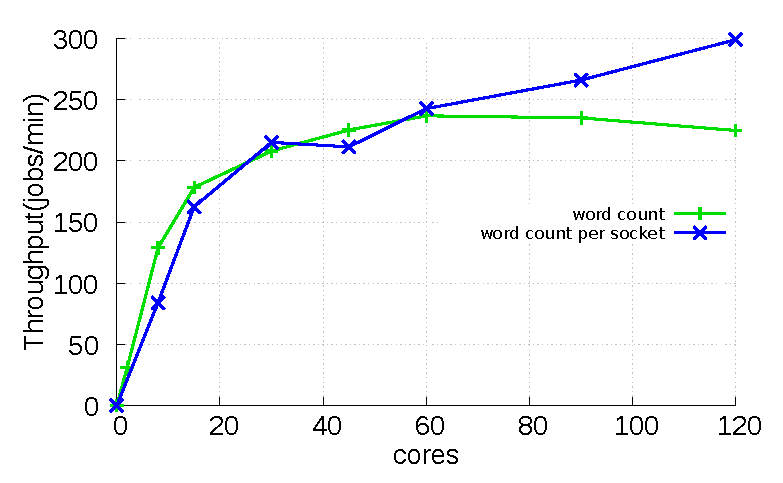
\includegraphics[width=1.8in]{graph/wc_docker.eps}
        \caption{Word Count}
    \end{subfigure}%
    \begin{subfigure}[b]{0.25\textwidth}
        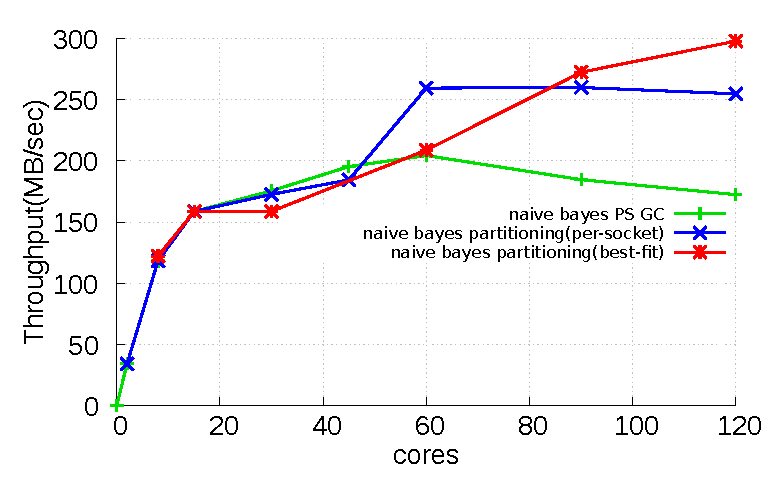
\includegraphics[width=1.8in]{graph/nb_docker.eps}
        \caption{Naive Basian}
    \end{subfigure}%
    \begin{subfigure}[b]{0.25\textwidth}
        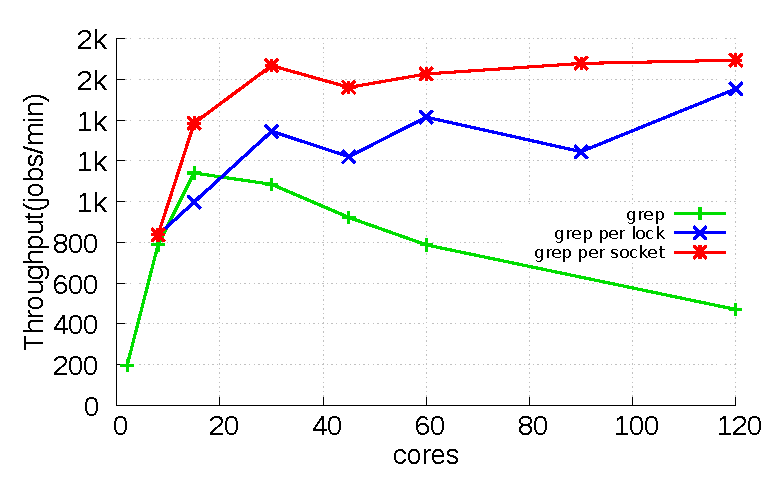
\includegraphics[width=1.8in]{graph/grep_docker.eps}
        \caption{Grep}
    \end{subfigure}%
    \begin{subfigure}[b]{0.25\textwidth}
        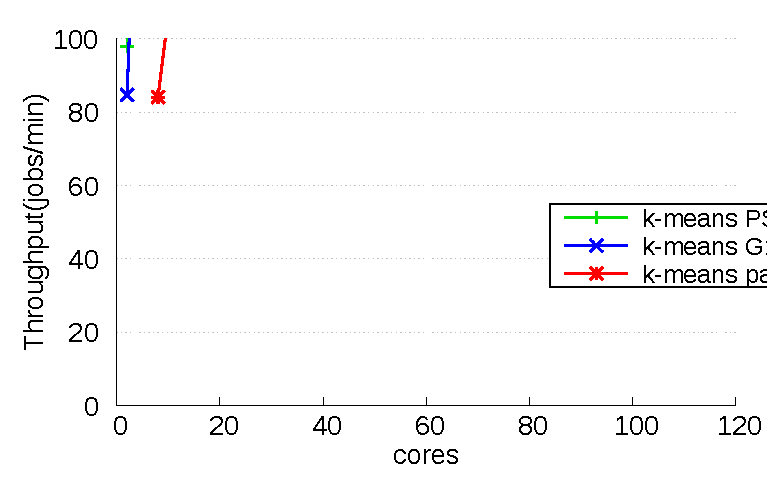
\includegraphics[width=1.8in]{graph/kmeans_docker.eps}
        \caption{K-means}
    \end{subfigure}%
    \caption{CPU utilization on 120 core.}
    \label{fig:docker}
\end{figure*}


\begin{figure*}[tb]
    \centering
    \begin{subfigure}[b]{0.25\textwidth}
        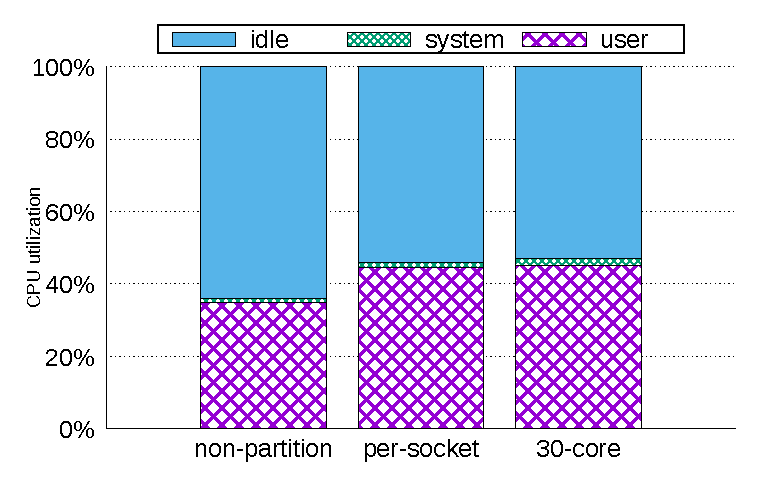
\includegraphics[width=1.8in]{graph/wc_cpuutils_docker.eps}
        \caption{Word Count}
    \end{subfigure}%
    \begin{subfigure}[b]{0.25\textwidth}
        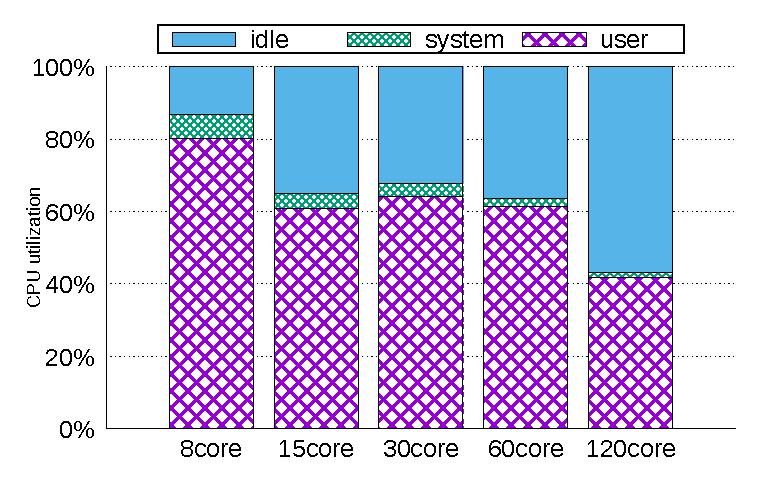
\includegraphics[width=1.8in]{graph/nb_cpuutils_docker.eps}
        \caption{Naive Basian}
    \end{subfigure}%
    \begin{subfigure}[b]{0.25\textwidth}
        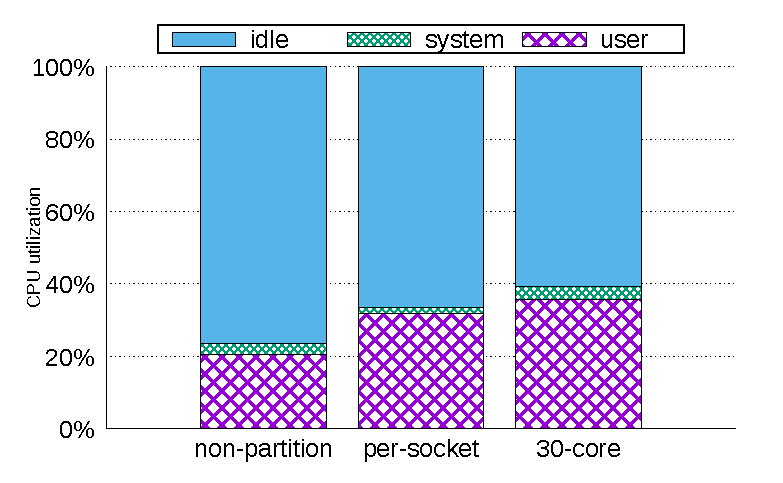
\includegraphics[width=1.8in]{graph/grep_cpuutils_docker.eps}
        \caption{Grep}
    \end{subfigure}%
    \begin{subfigure}[b]{0.25\textwidth}
        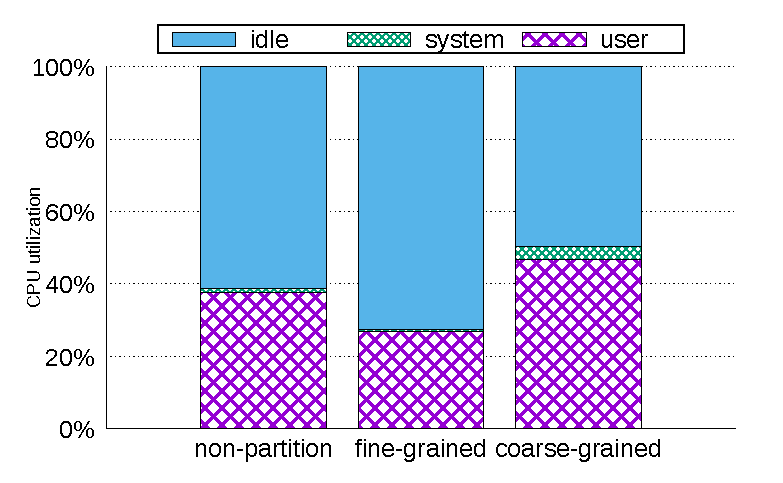
\includegraphics[width=1.8in]{graph/kmeans_cpuutils_docker.eps}
        \caption{}
    \end{subfigure}%
        \centering
    \caption{CPU utilization on 120 core.}
    \label{fig:utilization2}
\end{figure*}
